\documentclass[12pt]{scrartcl}
\usepackage{blubird}
% has options [nodate, nosans, nofancy, nocolor, code]

% box setup - should be moved to somewhere nicer
\mdfsetup{
	roundcorner = 2pt,
	linewidth = 1pt,
	innertopmargin = 0.5em,
	innerbottommargin = 1em,
	frametitlefont = \bfseries,
}

\usepackage{tikz}
\usetikzlibrary{snakes}

% TITLE
\title{Infinitely Many Proofs of Infinitely Many Primes}
\subtitle{(Special Thanks to Katherine Taylor, Forrest Hutchison, Emma Cardwell, Angela Zhao, HCSSiM 2019)}
\author{Bryan Lu}
\date{2 May 2022} % do not use if [nodate] option enabled

\begin{document}
\maketitle

\section{Classic Number Theory Proofs}
\subsection*{Proof by Euclid -- All}
Consider a finite list of primes $A,B,C$. Construct the line segment $DE$ such that $DE=A\cdot{B}\cdot{C}$. Construct $DF$ such that $DF=1$ and $D,E,F$ are collinear.
\begin{center}
	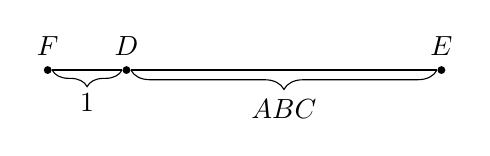
\begin{tikzpicture}
		\node (D) at (0,0) [label={$D$},fill=black,circle,inner sep =1pt] {};
		\node (E) at (4,0) [label={$E$},fill=black,circle,inner sep =1pt] {};
		\node (F) at (-1,0) [label={$F$},fill=black,circle,inner sep =1pt] {};
		\draw (F) -- (D) -- (E);

		\draw [decorate,decoration={brace,amplitude=7pt,mirror}]
		(D) -- (E) node [midway, below, yshift=-7pt]
		{$A{B}{C}$};

		\draw [decorate,decoration={brace,amplitude=6pt,mirror}]
		(F) -- (D) node [midway, below, yshift=-5pt]
		{1};

		%\draw [decorate,decoration={brace,amplitude=10pt, mirror}] (F) -- (E) node [midway, below, yshift=-10pt] {$\gamma$};
	\end{tikzpicture}
\end{center}
If $EF$ is prime, we have found a larger prime. If $EF$ is not prime, then it must divide some prime $G$. If $G$ is any of the primes $A,B,C$, then it must also divide $DF=1$. Since this isn't possible, $G$ must be a prime not in our list. Thus, we have found a new prime, and there are an infinite number of primes. Proof count: $1$.

\subsection*{Proof using Legendre's Formula (Whang, 2010) -- Ari}
Consider $n!$. Since prime factorization is unique, we may write $n! = \prod_{}{p^{N_p}}$, where $N_p = \lfloor \frac{n}{p} \rfloor + \lfloor \frac{n}{p^2} \rfloor + \lfloor \frac{n}{p^3} \rfloor + \cdot \cdot \cdot$ which is the number of times $p$ appears in $n!$. From this,
$$N_p \leq \frac{n}{p} + \frac{n}{p^2} + \frac{n}{p^3} + \cdot \cdot \cdot$$
By geometric series, $$ N_p \leq \frac{n}{p-1}$$
$$\prod{}{p^{N_p}} \leq \prod{}{p^{\frac{n}{p-1}}}$$
Separately, we know that $\frac{n}{2}^{\frac{n}{2}} \leq n!$ (which can be shown by induction), so we write $$\frac{n}{2}^{\frac{n}{2}} \leq (\prod{}{p^{\frac{1}{p-1}}})^n$$
$$\frac{n}{2}^{\frac{1}{2}} \leq \prod{}{p^{\frac{1}{p-1}}}$$
This can only be true for any $n$ if there are infinitely many primes. Proof count: $4$.

\subsection*{Proof (Folklore) -- Amber}
AFTSOC, let $p$ be the largest prime. $\exists$ a prime $q$ s.t. $q\mid{2^p-1}.$
Consider the multiplicative group mod $q$ $(\ZZ/q\ZZ)^\times.$
We know that $o(2)\mid{p}$, but since $p$ is prime and $o(2)\neq{1},$ $o(2)=p$.By Fermat's Little Theorem, $p\mid{q-1}$, so $q>p$, which is a contradiction. So, there is no largest prime $p$ and thus an infinite number of primes. Proof count: $6$.


\subsection*{Proof using Combinatorics (the Incompressibility Method) -- Milo}
AFTSOC there are finitely many primes, $p_1, p_2, ..., p_n$. $\forall n \in \mathbb{Z}^+, n = p_1^{e_1}p_2^{e_2}...p_k^{e_k}$. There are $n$ numbers between $1$ and $n$. Each $e_i$ can be at most $\log_2n$, so there are $1+\log_2n$ options for each exponent. This gives at most $(1+\log_2n)^k$ possible prime factorizations for numbers between 1 and $n$. For ease of computation, consider $n = 2^{m-1}$. Then there are $2^{m-1}$ numbers between 1 and $n$, and $(1+\log_2 2^{m-1})^k = m^k$ possible prime factorizations. For large enough $m$, there are not enough prime factorizations than there are numbers, a contradiction. Therefore, there are infinitely many primes. Proof count: $5$.

\subsection*{Proof of Infinite Proofs by Paul}
According to Bertrand's postulate, we are guaranteed to find at least one prime between $n$ and $2n$ for any $n \in \mathbb{Z}^+$. Since we can start at any $n$ and there are an infinite number of places to start at, we have an infinite number of primes! Proof count: $11+\infty+\infty\cdot\infty+\infty$


\subsection*{Proof with Topology (F\"urstenburg) -- David}
Call $U \subset \mathbb{Z}$ \textit{nepo} if if $U = \emptyset$ or $U$ is a union of sets of the form $S(a, b) = \{ x \in \mathbb{Z} : x \equiv b \pmod{a}$. In other words, every element of $U$ is in an arithmetic progression. \\

Why is this a topology? Just need to check finite intersections of open sets is open.

%should we format the lemmas the official way?
\textbf{Lemma 1:} The intersection of finitely many nepo sets is nepo. \\
\textbf{Proof:} Let $U_1, U_2, ... U_n$ be nepo. Let $x \in U_1 \cap U_2 \cap ... \cap U_n$. Since $x \in U_1$, $x \in S(a_1, x) \subset U_1$. Since $x \in U_2$, $x \in S(a_2, x) \subset U_2$, and so on. Let $a = lcm(a_1, a_2, ... a_n)$. Then $S(a, x) \subset S(a_1, x) \subset U_1$, $S(a, x) \subset S(a_2, x) \subset U_2$ and so on. Now we have $S(a,x) \subset U_1 \cap U_2 \cap ... \cap U_n$, so $U_1 \cap U_2 \cap ... \cap U_n$ is nepo.

Consider $S(p, 0)$, the set of all integer multiples of $p$. Now consider $\{1, -1\}$, the only members of $\mathbb{Z}$ that aren't multiples of primes.

$\braces{-1,1}$ is open, but this is impossible.


Call a set $V \subset \mathbb{Z}$ \textit{desolc} iff its complement is nepo. \\
\textbf{Lemma 2:} The union of finitely many desolc sets is desolc. \\
\textbf{Proof:} Let $V_1, V_2, ... V_n$ be desolc. $(V_1 \cup V_2 \cup ... \cup V_n)^c = V_1^c \cap V_2^c \cap ... \cap V_n^c$, which is the intersection of finitely many nepo sets and therefore nepo. So, its complement, or $V_1 \cup V_2 \cup ... \cup V_n$, is desolc.\\
Consider $S(p, 0)$, the set of all integer multiples of $p$. Now consider $\{1, -1\}$, the only members of $\mathbb{Z}$ that aren't multiples of primes. This set isn't nepo, so its complement can't be desolc. We can write this non-desolc set as $\mathbb{Z} \setminus \{1, -1\} = \bigcup_{p \textrm{ prime}}S(p, 0)$. But for a given $p$, $S(p, 0)$ is desolc. If there were finitely many primes, $\mathbb{Z} \setminus \{1, -1\}$ would be the union of finitely many desolc sets, so it would be desolc. Since we know that's not true, there must be infinitely many primes. Proof count: 7.

\subsection*{Proof with Analysis (Erd\"os) -- Kelly}
We will show that $\sum_{p}{\frac{1}{p}}$, where $p$ ranges over all primes, diverges. Suppose that the series converges to some value. Then $\exists k $ such that $$\frac{1}{p_{k+1}} + \frac{1}{p_{k+2}} + \frac{1}{p_{k+3}} + ... < \frac{1}{2}$$
Let's call all primes from $p_{k+1}$ on up ``big primes" and the primes from $p_1$ to $p_k$ ``small primes". Now we take some $n \in \mathbb{N}$ and count the number of numbers less than or equal $n$ in two ways. First, just by counting, we get that there are $n$ of them. Then, we'll count first the number of numbers less than $n$ that only have small prime factors (call this total $i$), and add that to the number of numbers with at least one big prime factor (call this total $j$). Note that for any prime $p$ the number of numbers $\leq n$ with $p$ as a factor is $\lfloor \frac{n}{p} \rfloor$. Therefore, we know that $$ j \leq \frac{n}{p_{k+1}} + \frac{n}{p_{k+2}} + \frac{n}{p_{k+3}} + ... = n(\frac{1}{p_{k+1}} + \frac{1}{p_{k+2}} + \frac{1}{p_{k+3}} + ...) < \frac{n}{2}$$
Now we'll consider some $m \leq n$ with only small prime factors. We write $m$ in the form $w^2x$, where $x$ contains no squares as factors. This means none of the $k$ possible prime factors can appear in $x$'s factorization more than once, giving $2^k$ possibilities for the value of $x$. Since $w < \sqrt{n}$, we have $ i \leq 2^k \sqrt{n}$. The square root function grows more slowly than $\frac{n}{2}$, so $i < \frac{n}{2}$ for sufficiently large $n$. Putting it all together, $i+j = (\textrm{number of numbers less than or equal to n}) < \frac{n}{2} + \frac{n}{2} = n$. This is a contradiction. Therefore, $\sum_{p}{\frac{1}{p}}$ diverges, so there must be infinitely many terms in the series, so there must be infinitely many primes. Proof count: $8$.

\subsection*{Proof using the Prime Number Theorem }
Well known that $\pi(x)$, the number of primes $\leq x$, grows asymptotically as $\frac x{\ln x}$.


% \subsection*{Proof by Jessica (2)}
% We will run an experiment.\\
% \begin{multicols}{2}
% 	$3$-prime\\
% 	$5$-prime\\
% 	$7$-prime\\
% 	$9$-experimental error\\
% 	$11$-prime\\
% 	$13$-prime\\
% 	$15$-experimental error\\
% 	$17$-prime (very)\\
% \end{multicols}
% Thus, every odd number is prime, except for the experimental errors. Since there are an infinite number of odd numbers, there are an infinite number of primes.

% \subsection*{Proof by Paul}
% Let's look at the arithmetic progression $a, a+d, a+2d, ... d \in \mathbb{Z}^+$. According to the Van der Waerden theorem, it is always possible to color the integers with finitely many colors in a way that produces monochromatic arithmetic progressions of any desired length. According to Fermat's theorem, no arithmetic progression has more than 3 perfect squares in a row.
% \newline
% Claim: $|\mathbb{P}| = +\infty$
% \newline
% Proof: Let $P = \{p_1, p_2, ..., p_n\}$ be a finite set of primes. Define a function $c: \mathbb{Z}^+ \longrightarrow$ binary, where the $k^{\textrm{th}}$ bit is a 1 if $p_k$ has an odd power in the prime factorization of $n$ and 0 otherwise.
% \newline
% We can find $A, A+2D, A+3D$ all of the same color, so they all have the same square free part. If they contain a prime not in our list, we've found a new prime.
% \newline
% $R = \textrm{square free}$
% $\frac{A}{R}, \frac{A+D}{R}, \frac{A+2D}{R}, \frac{A+3D}{R}$
% $d = D/R$
% then we have 4 squares in a row, a contradiction of Fermat's theorem. Thus, we proved there are an infinite number of primes. Proof count: $9$.

% \subsection*{Proof by David (2)}
% We assume for the sake of contradiction that there are finitely many primes.

% By the proof that Paul just gave, there exist infinitely many primes. This gives a contradiction, so our assumption that there are finitely many primes is false. Thus there are infinitely many primes.

\subsection*{Proof by Construction -- Greg}
We'll consider the series $F_0, F_1,...$ such that $F_n = 2^{2^n}+1$. \\
\textbf{Lemma:} $\prod^{n-1}_{i=0}{F_i} = F_n - 2$.\\
\textbf{Proof:} We will use induction. Assume FTSOC that the relation holds $\forall i$ s.t. $0 < i < n$. Then $$\prod^{n}_{i=0}{F_i} = F_n \cdot \prod^{n-1}_{i=0}{F_i} = (2^{2^n}+1)\cdot((2^{2^n}+1)-2) = 2^{2^n}\cdot2^{2^n} - 1 = F_{n+1}-2$$
Now we wish to show that for any $i, j$ s.t. $i \neq j$, $F_i$ and $F_j$ are relatively prime. WLOG, $j > i$. Let $d = gcd(F_i, F_j)$. Since $d | F_j$, $d | (\prod^{j-1}_{k=0}F_k + 2)$. We know $d | \prod^{j-1}_{k=0}F_k$ since $d | F_i$, so $d | 2 \implies d = 2$ or $d = 1$. But all the $F_n$ are odd, so $d=1$. Now we must have an infinite sequence of relatively prime numbers, which is only possible if we have infinitely many primes at our disposal. Proof count: 10.

\subsection*{Proof of Infinite Proofs by Amber}
Let's look at
\begin{equation*}
	17, \hspace{0.3em} 17+1,  \hspace{0.3em} 17(17+1)+1, \hspace{0.3em}  17(17+1)\Big(17(17+1)+1\Big)+1,...
\end{equation*}
Each term is generated by multiplying the previous term by $17$, then adding 1. Because all of the terms are relatively prime to each other, there must be a new prime for each new term in our list. We can extend this to all $n>1, n \in \mathbb{N}$, and this gives us an infinite number of ways to show that there are an infinite number of primes:
\begin{equation*}
	n, \hspace{0.3em} n+1, \hspace{0.3em} n(n+1)+1, \hspace{0.3em}  n(n+1)\Big(n(n+1)+1\Big)+1,...
\end{equation*}
We can further generalize this by considering any pair of numbers $a,b$ where gcd$(a,b)$ = 1. We can construct a sequence of terms each relatively prime to the others by multiplying together all of the previous terms together:
\begin{equation*}
	a, \hspace{0.3em} a+b, \hspace{0.3em} a(a+b)+b, \hspace{0.3em}  a(a+b)\Big(a(a+b)+b\Big)+b,...
\end{equation*}
We've found an infinite number of ways to construct infinite sequences that prove there are an infinite number of primes. Proof count: $11+\infty+\infty\cdot\infty$



% \subsection*{Proof by Jessie (2)}
% AFTSOC that there are finitely many primes. We know that not all integers are prime, but we will use induction to show that all integers are prime anyway.
% \newline
% Base case: 0 \checkmark
% \newline
% IHOP: for all $n, n \neq 0, n+1$ is prime. The formal inductive proof is left to the audience, but these examples work, so everything else \textit{obviously} should work.
% \newline
% Case 1: $n = 1 \longrightarrow n+1 = 2$ \checkmark
% \newline
% Case 2: $n=2 \longrightarrow n+1 = 3$ \checkmark
% \newline
% Therefore all integers are prime, so there are infinitely many primes. This contradicts our assumption, so our assumption is wrong. Therefore, there are an infinite number of primes.

% Note from Jessica:\\
% AFTSOC induction doesn't work like this. \\
% Contradiction: there are infinitely many primes.
\section*{Infinitude of Specific Classes of Primes}

\subsection*{Proof (Folklore) -- Jessica}
We'll prove that there are infinitely many primes congruent to $3\pmod{4}$. Let $f_1, f_2, ... f_k$ be a list of primes of this form. Let $N = 4 f_1 f_2 \cdot \cdot \cdot f_k - 1$. Note that $N \equiv 3 \pmod{4}$. Either $N$ is prime or $N$ is composite. If $N$ is prime, we're done - we've found a prime $\equiv 3 \pmod{4}$ that's not on our list. If $N$ is composite, it must have some prime factor $\equiv 3 \pmod{4}$, even though it's relatively prime to everything in our list. Therefore, we've found a new prime $\equiv 3 \pmod{4}$. So, there are infinitely many primes.
Proof count: $2$.


\subsection*{Proof by Jessie}
We will show that there are infintely many primes of the form $p=4k+1$. Let $N=(n!)^2+1$ for $n>1$, and note that the smallest prime $p \mid N$ is some $p > n, p \neq 2$.
Then,
\begin{center}
	$N=0$ (mod $p$)\\
	$(n!)^2+1\equiv0$ (mod $p$)\\
	$(n!)^2\equiv-1$ (mod $p$)\\
	$(n!)^{p-1}\equiv(-1)^{\frac{p-1}{2}}$ (mod $p$)\\
\end{center}
By Fermat's,
\begin{center}
	$1\equiv(-1)^{\frac{p-1}{2}}$ (mod $p$)
\end{center}
Thus, $\frac{p-1}{2}=2k$, so $p=4k+1$. This means we can generate a new prime for any $n$, so there are infinitely many primes. Proof count: $3$.

\subsection*{Proof using Dirichlet's Theorem for Arithmetic Progressions}
For any two positive coprime integers $a$ and $d$, there are infinitely many primes of the form $a + nd$, where $n$ is also a positive integer. In other words, there are infinitely many primes that are congruent to $a \mod d$.

Case where $a = 1$:


\subsection*{Proof by Paul (2)}
Counting by Cerruti and Murun:\\
Legendre Function:\\
$$\phi{(x,y)} = \lvert \left\{n \mid n\leq x, n \text{ has no prime factors} \leq y \right\} \rvert $$
Claim:
$$\pi(x)= \pi(\sqrt{x}) + \phi{(x,\sqrt{x})} - 1.$$\\
Let $p_1,p_2,...,p_k$ be all the primes $ \leq y$. By PIE,
$$\phi{(x,y)}=x-\sum{\left\lfloor\frac{x}{p_i}\right\rfloor}+\sum{\left\lfloor\frac{x}{p_ip_j}\right\rfloor}+\cdots+(-1)^n \left\lfloor \frac{x}{p_1p_2\cdots p_k}\right\rfloor$$
If we let $N=p_1p_2\cdots{p_k}$, and this includes every prime, then
$$L=\phi{(N^2,N)}=N^2-\sum{\left\lfloor\frac{N^2}{p_i}\right\rfloor}+\sum{\left\lfloor\frac{N^2}{p_ip_j}\right\rfloor}+\cdots+(-1)^n \left\lfloor \frac{N^2}{p_1p_2\cdots p_k}\right\rfloor=mN.$$
So every prime divides $1$, which is a contradiction. Proof count: $11$.


\subsection*{Proof of Infinite Proofs by Cailan:}
Let's consider the Riemann zeta function:

\begin{equation*}
	\zeta(s) = \sum_{n=1}^\infty \frac{1}{n}s = \frac{1}{1s} + \frac{1}{2s} + \frac{1}{3s} + ... + \frac{1}{p_1^{e1}...p_k^{ek}s} + ...
\end{equation*}
By Unique Prime Factorization, we can represent each $n$ as a product of primes to the power of primes, $p_1^{e1}...p_k^{ek}$. We can represent the entire sum as the product of many geometric sequences:
\begin{equation*}
	\zeta(s) =(1 + {\frac{1}{2s}} + \frac{1}{2^2s}+...)(1 + \frac{1}{3s}+\frac{1}{3^3s}+...)...(1 + \frac{1}{ps}+\frac{1}{p^ps}+...)
	=\Pi_{p\textrm{ prime}}(1-\frac{1}{p^{s}})^{-1}
\end{equation*}
Now, AFTSOC there are finitely many primes. For $s=1$, the left hand side of the Riemann zeta function diverges. However, the right hand side is a bunch of geometric sequences, each with a common ratio $r = \frac{1}{p^s}$. The product of converging geometric sequences is finite, so the right hand side is finite. This contradicts the left hand side, which diverges, thus there are infinitely many primes.
\newline
\newline
Recall $\forall k \in \mathbb{Z}^+$ at $s=2k$, where $B$ is a Bernoulli number:
\begin{equation*}
	\Pi_{p\textrm{ prime}}(1-\frac{1}{p^{2k}})^{-1} = \zeta(2k) = \frac{(-1)^{k+1}B_{2k}(2\pi)^{2k}}{2(2k!)}
\end{equation*}
AFTSOC that there are finitely many primes. Then, the left hand side is rational. However, $\pi$ is transcendental, so the right hand side can't be rational. This is a contradiction, therefore there are infinitely many primes. Proof count: $11+\infty$


\end{document}